\documentclass{article}

\usepackage{Engineering}
\pdftitle{Electrical-eng}

% === TEXT ===
\title{\textbf{Electrical Engineering \\ HSLU, Semester 2}}
\author{Matteo Frongillo}
\date{}

\begin{document}

\maketitle
\tableofcontents
\pagebreak

\part{...}
\section{...}
\subsection{Current strength or current ``I''}
\begin{center}
    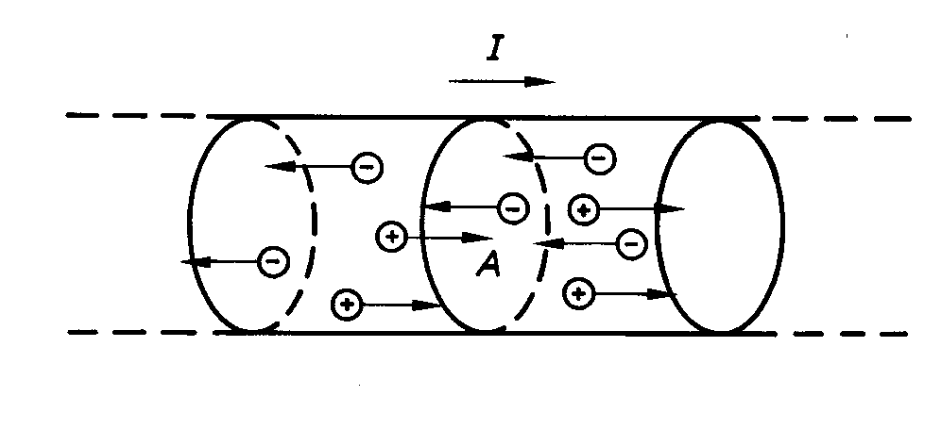
\includegraphics[width=.4\textwidth]{media/intensity.png}
\end{center}
\[I\ [A] =\dfrac{\text{el. charge}}{t}\]

\subsection{Current density ``J''}
\begin{center}
    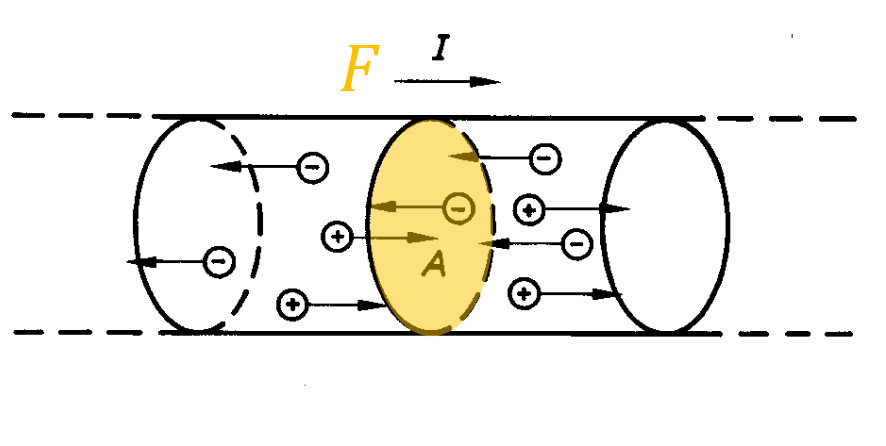
\includegraphics[width=.4\textwidth]{media/density.png}
\end{center}
The current density indicates how large the current per cross-sectional area (F) is:
\[J\ [\dfrac{A}{mm^2}] = \dfrac{I}{F}\]

\subsection{Temperature dependence of the resistance}
\begin{center}
    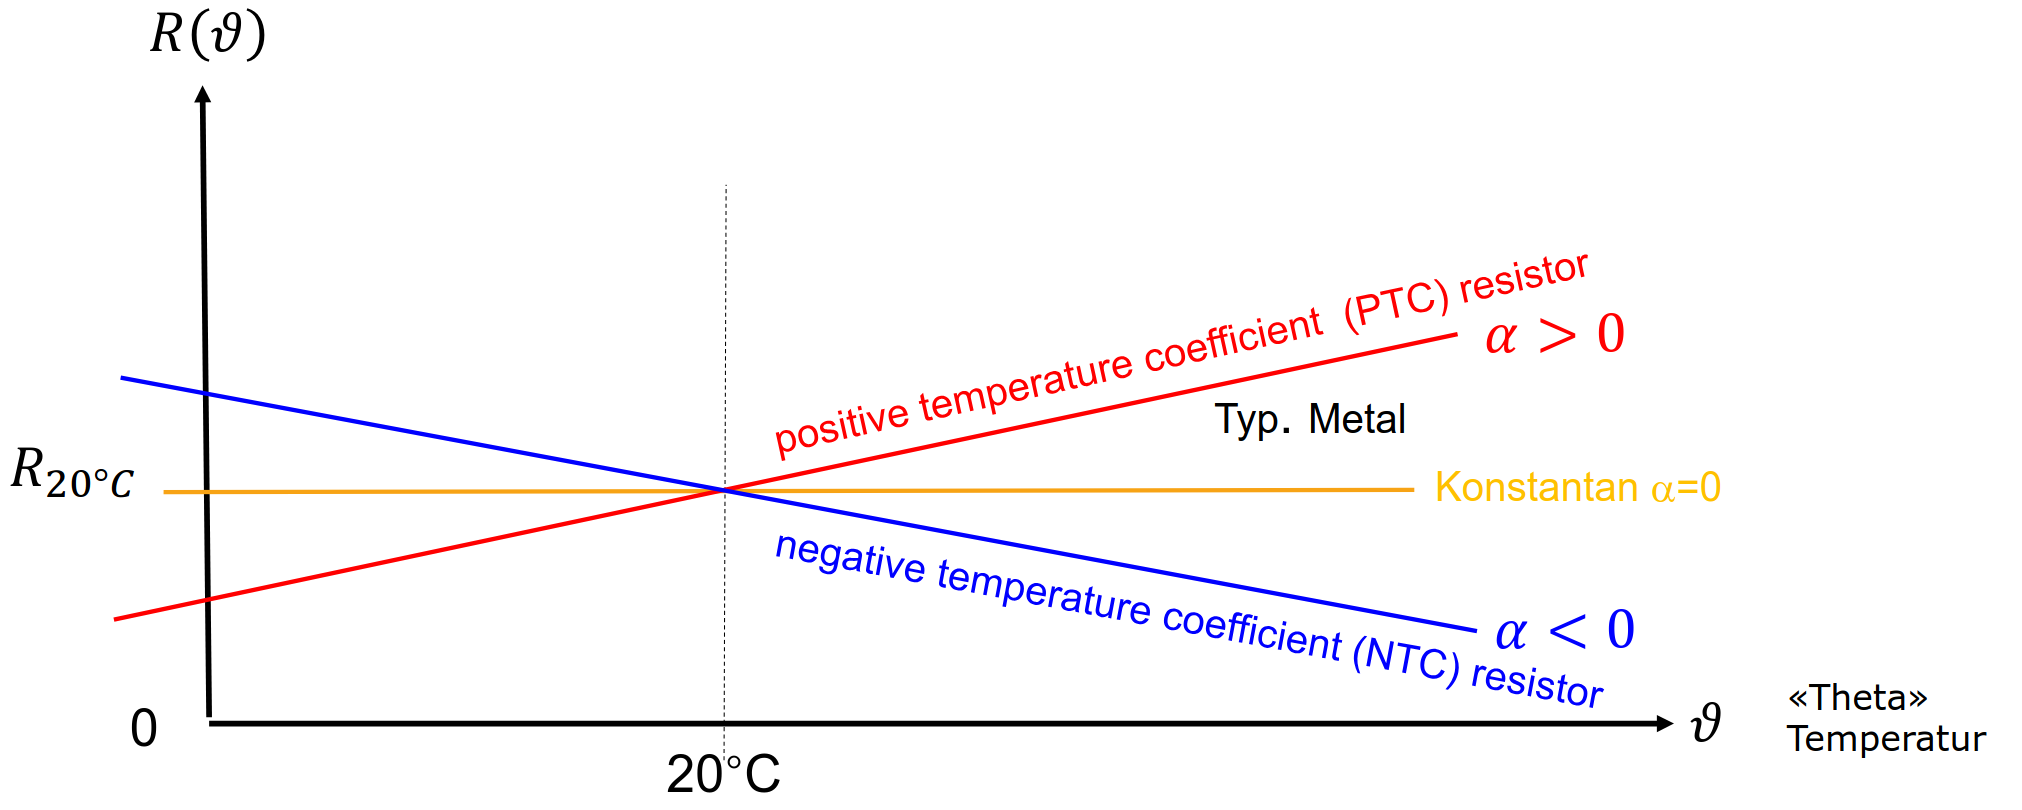
\includegraphics[width=\textwidth]{media/resistance.png}
\end{center}
Depending on the material, the resistance can increase, remain the same or decrease with temperature. In
ET+L we calculate using the linear approach.
\figbox{$R(\vartheta) = R_{20}(1+\alpha(\vartheta-20^{\circ}\text{C})) = R_{20}(1+\alpha \Delta T)$}

\subsection{Object properties}
The resistance indicates the voltage required for a
current. In addition to the material, the cross-sectional
area and also the length are decisive factors.
\[R=\frac{U}{I}\]

\subsection{Reciprocal quantities}
\subsubsection{Specific resistance}
To describe material properties, the resistance per length
and cross-sectional area is specified (precondition:
homogeneous conductor, direct current):
\[\rho\ [\frac{\Omega \cdot mm^2}{m}] = R\cdot \frac{A}{l}\]

\subsubsection{Conductance}


\subsubsection{Specific conductivity}




\end{document}
